% Этот шаблон документа разработан в 2014 году
% Данилом Фёдоровых (danil@fedorovykh.ru) 
% для использования в курсе 
% <<Документы и презентации в \LaTeX>>, записанном НИУ ВШЭ
% для Coursera.org: http://coursera.org/course/latex .
% Исходная версия шаблона --- 
% https://www.writelatex.com/coursera/latex/2

\documentclass[../main.tex]{subfiles}

%%% Работа с русским языком
\usepackage{cmap}					% поиск в PDF
\usepackage{mathtext} 				% русские буквы в формулах
\usepackage[T2A]{fontenc}			% кодировка
\usepackage[utf8]{inputenc}			% кодировка исходного текста
\usepackage[english,russian]{babel}	% локализация и переносы

%%% Дополнительная работа с математикой
\usepackage{amsfonts,amssymb,amsthm,mathtools} % AMS
\usepackage{amsmath}
\usepackage{icomma} % "Умная" запятая: $0,2$ --- число, $0, 2$ --- перечисление

%% Номера формул
%\mathtoolsset{showonlyrefs=true} % Показывать номера только у тех формул, на которые есть \eqref{} в тексте.
%% Шрифты
\usepackage{euscript}	 % Шрифт Евклид
\usepackage{mathrsfs} % Красивый матшрифт

%% Свои команды
\DeclareMathOperator{\sgn}{\mathop{sgn}}

%% Перенос знаков в формулах (по Львовскому)
\newcommand*{\hm}[1]{#1\nobreak\discretionary{}
	{\hbox{$\mathsurround=0pt #1$}}{}}

%%% Работа с картинками
\usepackage{graphicx}  % Для вставки рисунков
\graphicspath{{images/1/}{images/2/}{{images/4/}}}  % папки с картинками
\setlength\fboxsep{3pt} % Отступ рамки \fbox{} от рисунка
\setlength\fboxrule{1pt} % Толщина линий рамки \fbox{}
\usepackage{wrapfig} % Обтекание рисунков и таблиц текстом

%%% Работа с таблицами
\usepackage{array,tabularx,tabulary,booktabs} % Дополнительная работа с таблицами
\usepackage{longtable}  % Длинные таблицы
\usepackage{multirow} % Слияние строк в таблице


\usepackage{indentfirst}
\usepackage{hyperref}
\usepackage{booktabs}
\usepackage{float}
\usepackage[table]{xcolor}

% код в matlab
\usepackage{matlab-prettifier}
\usepackage{listings,lstautogobble}
\lstset{autogobble=true}


\begin{document} % конец преамбулы, начало документа
	В данной главе будет использован метод имитиации отжига для минимизации следующей функции
	\[f(x) = x^2 (2 + |\sin4x|), x \in \mathbb{R}\]
	
	Построим ее график:
	\begin{figure}[H]
		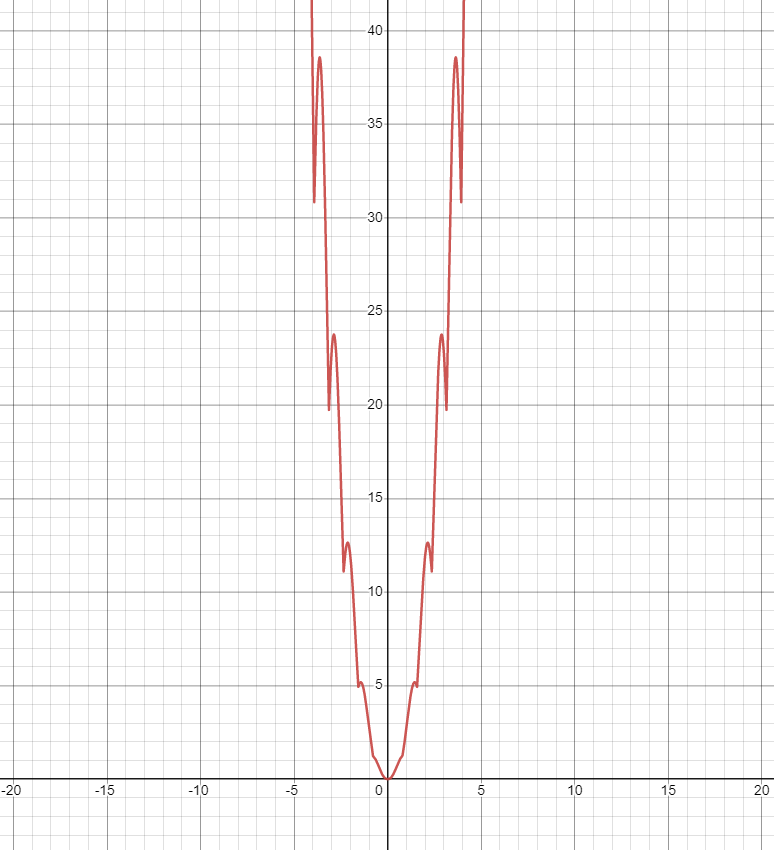
\includegraphics[width = 0.7\textwidth]{ann_3}
	\end{figure}
	
	
	
	Очевидно, что ее глобальный минимум равен нулю, и он достигается при $x=0$. 
	
	Теперь опишем детали применения алгоритма имитации отжига к данной задаче. Преобразование точки $x$ для получения новой точки $x'$ будет иметь следующий вид:
	\[x' = x + \xi, \text{ где }\xi \sim U[-1, 1]\]
	
	Начальное приближение $x_0$ будет браться из равномерного распределения на отрезке $[-10, 10]$, то есть
	
	\[x_0 \sim U[-10, 10]\]
	
	В качестве критерия останова будет выступать достижение температурой близкого к нулю значения. 
	
	Тогда код алгоритма имитации отжига будет иметь следующий вид:
	
	\begin{lstlisting}[
		frame=single,
		numbers=left,
		style=Matlab-Pyglike]
		function [x, y] = annealing_alg(alpha, t_0, t_thr)
		t = t_0;
		x = unifrnd(-10, 10);
		y = x^2 * (2 + abs(sin(4 * x)));
		while t > t_thr
		  x_new = x + unifrnd(-1, 1);
		  y_new = x_new^2 * (2 + abs(sin(4 * x_new)));
		  delta_y = y_new - y;
		  p = exp(-delta_y / t);
		  xi = binornd(1, p);
		  if or(delta_y < 0, xi == 1)
		    x = x_new;
		    y = y_new;
		  end
		  t = t * alpha;
		end
	\end{lstlisting}
	
	Возьмем значения параметров, которые были использованы на лекции Шамина, то есть начальную температуру положим равной 100, нижнюю границу температуры - $10^{-10}$, а также пусть $\alpha=0.95$. Запустим несколько раз наш алгоритм:
	
	\begin{lstlisting}[
		frame=single,
		numbers=left,
		style=Matlab-Pyglike]
		[x, y] = annealing_alg(0.95, 100, 10^(-10))
		
		x =
		
		0.0022
		
		
		y =
		
		9.6014e-06
		
		>> [x, y] = annealing_alg(0.95, 100, 10^(-10))
		
		x =
		
		-1.2132e-04
		
		
		y =
		
		2.9446e-08
		
		>> [x, y] = annealing_alg(0.95, 100, 10^(-10))
		
		x =
		
		-0.0177
		
		
		y =
		
		6.4701e-04
		
		>> 
	\end{lstlisting}
	
	Во всех тестах оптимальная точка колеблется около нуля, который является точкой глобального минимума целевой функции. Также каждая из итераций была выполнена достаточно быстро.
	
	Таким образом, несмотря на то, что алгоритм имитации отжига и не нашел точный глобальный минимум, он подобрался к нему достаточно близко, при этом сделал это довольно быстро.
	
	
\end{document} % конец документа